
\section{Comparison of Different Multiplier Structures}
\subsection{Standard Binary Multiplier}

\subsection{Online Multiplier}
\subsubsection{Algorithm}
Similar to online addition, online multiplication can also be implemented in a unrolled digit-parallel manner, of which the optimized algorithm is shown in Algorithm~\ref{Algorithm:OM_DigitParallel} [xxx]. In this algorithm, both inputs and outputs are $N$-digit numbers as given in (\ref{Eq:Online_Operands}). For a given iteration $j$, the product digit $z_j$ is generated MSD-first through a selection function $sel()$. For any radix $r$ and chosen digit set, there exits an appropriate selection method and a value of $\delta$ which ensure convergence. As the binary radix is used most commonly in computer arithmetic, we keep $r=2$ throughout this paper with the corresponding redundant digit set $\{\overline{1},0,1\}$. In this case $sel()$ is given by (\ref{Eq:SelFunc_OM})~\cite{Ercegovac_OnlineMult}.

\begin{algorithm}[tbp]
  \caption{Digit Parallel Online Multiplication}\label{Algorithm:OM_DigitParallel}
  \begin{algorithmic}[1]
    \State \textbf{Initialization:} $P_{[0]}=0$                     \vspace{.5ex}
    \For{$j=1,~2,~\cdots,~N$}                                       \vspace{.5ex}
        \State $Xy_j \leftarrow X \cdot y_j$                        \vspace{.5ex}
        \State $W_{[j]}    \leftarrow  P_{[j-1]} + Xy_j$            \vspace{.5ex}
        \State $z_{j}  ~~      \leftarrow  sel(W_{[j]})$            \vspace{.5ex}
        \State $P_{[j+1]}  \leftarrow  r\left(W_{[j]}-Z_{[j]}\right)$   \vspace{.5ex}
    \EndFor                                                         \vspace{.5ex}
    \State $Z_{[N+1:2N]} \leftarrow frac(W_{[N]})$                  \vspace{.5ex}
  \end{algorithmic}
  \vspace{-1ex}
\end{algorithm}

\begin{eqnarray}\label{Eq:SelFunc_OM}
\small
  sel(W_{[j]})=\begin{cases}
    1 & \text{ if } W_{[j]} \geqslant \frac{1}{2} \\
    0 & \text{ if } -\frac{1}{2}\leqslant W_{[j]}<\frac{1}{2} \\
    \overline{1} & \text{ if } W_{[j]}<-\frac{1}{2}
  \end{cases}
\normalsize
\end{eqnarray}

The parallel implementation of Algorithm~\ref{Algorithm:OM_DigitParallel} is illustrated in Fig.~\ref{Fig:PM} where $N=4$. The details of implementation are addressed in our previous work [xxx].

\begin{figure}[tbp]
  \centering
  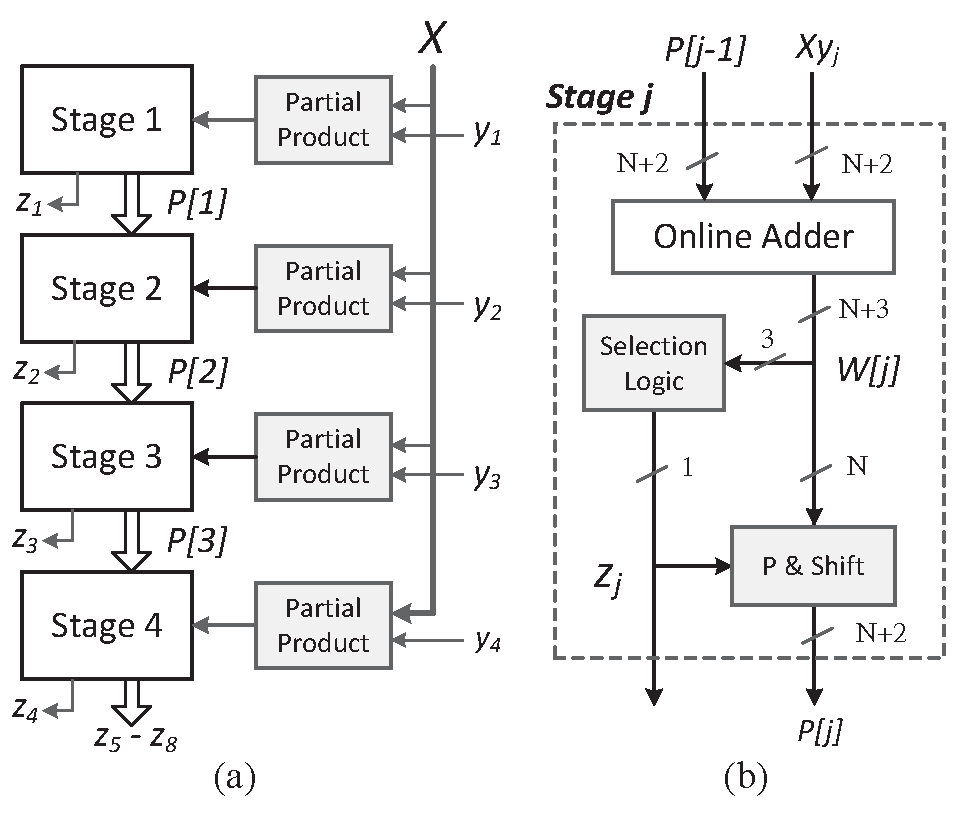
\includegraphics[width=.42\textwidth]{./figures/ParallelMult_Structure.eps}
  \caption{(a) Structure of a 4-digit online multiplier. (b) Structure of one stage. The word-length of all signals are labeled in digits, $N$ is the word-length of input signals.}
    \vspace{-2ex}
  \label{Fig:PM}
\end{figure}

\subsubsection{Structure Optimization for Half Precision Results}
In actual applications, normally the multiplier is connected with other arithmetic operators. If the multiplication result is utilized for subsequent operations, and a consistent word-length is used throughout the system, then only the most significant half of the product is required. In a conventional multiplier with standard binary arithmetic, this is achieved by either truncating or rounding the least significant half of the products. However, both the computation time and the structure remains unchanged, because results are generated from LSDs.

In comparison, OM offers the flexibility to simplify the structure corresponding to the required precision. This is possible because in an OM, the product digits are generated initially from the MSD, and there is no carry propagation from the LSD to the MSD with the employment of the redundant number system. This will potentially lead to a more area efficient design. For example, the modified structure diagram of a 4-digit OM is illustrated in Fig.~\ref{Fig:PM_half}(a). The word-length of signals within each stage can be correspondingly reduced, as shown in Fig.~\ref{Fig:PM_half}(b). Notice that instead of keeping identical word-length throughout the stages (in Fig.~\ref{Fig:PM}), in the modified structure the signal word-lengths depend on the stage number $j$ and hence fewer bits of signals are needed for LSD stages.

\begin{figure}[tbp]
  \centering
  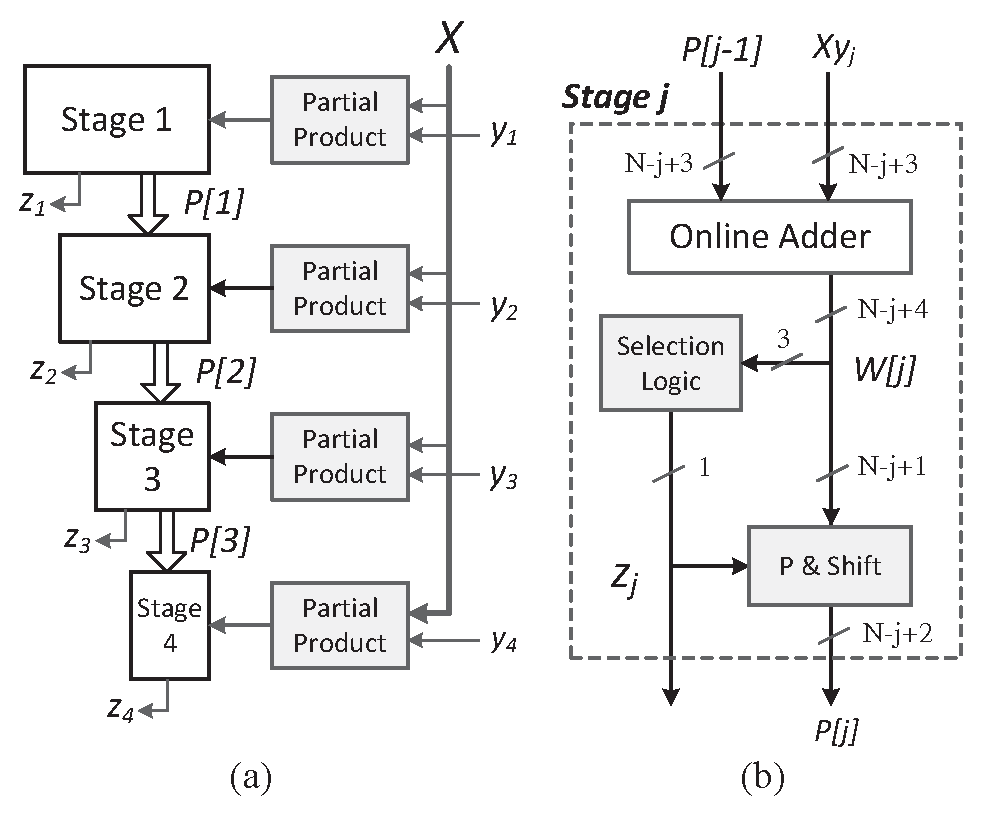
\includegraphics[width=.42\textwidth]{./figures/ParallelMult_MSDhalf.eps}
  \caption{(a) A 4-digit online multiplier with half precision results. (b) Structure of stage $j$, with the word-length of all signals labeled.}
    \vspace{-2ex}
  \label{Fig:PM_half}
\end{figure}
